\chapter[Project Planning]{Project Planning}

% \section{Methodology}
% https://zube.io/blog/agile-project-management-workflow-for-github-issues/
\section{Introduction}
As this project was initially the idea of its project partner who needed an interactive frontend application, planning the project had to be adapted accordingly. This chapter will give an overview about which parts of the whole system are already provided for and identifies the requirements and potential solutions for the frontend.

The main idea is to give tenants, proprietors and facility management a way to communicate over a single point of access. In its first version, they should be able to discuss topics they care about, easily make announcements, submit and track the state of maintenance issues and to create polls in order to provide an easy way for decision-making. It is meant to move traditional house management to the 21st century.

% Talk about project idea in more detail
\section{Provided Services}
% DB - postgresql
% API - documented with postman
The Database and API are both provided by the project partner. The first is a PostgreSQL instance, the latter an API built on top of Django and Django Rest Framework. These two technologies reflect the backend of the system as a whole. The API is documented with Postman, describing each endpoint in terms of what type of data has to be sent and what data will be returned. Apart from making these compatible with a containerized environment (see \autoref{ch:deployment}), no further action has to be taken in order to use these services.

\section{Requirements}
% List requirements defined by project partner
% write these as user stories
% illustrate as Use Case diagram
The requirements of the application are primarily defined by the project partner. These are:
\begin{itemize}
    \item Digital Noticeboard
    \item Polls
    \item Forum
    \item Issue Management    
\end{itemize}

\subsection{Digital Noticeboard}
The digital noticeboard is what it says: a noticeboard accessible online. It is a unidirectional way of communication between house parties. A typical example would be to announce a get-together everyone is invited to. \newline
Allowed user roles: Proprietors, Tenants, Facility Managament

\subsection{Polls}
Polls are intended to remove the friction of decision-making. An example would be a facade that has to be repainted with a new color. To get an initial idea which color it should be, Proprietors can create polls and let other proprietors choose between given options. \newline
Allowed user roles: Proprietors

\subsection{Forum}
The Forum is a way of discussing topics related to a specific house. E.g. a tenant wants to know when garbage cans are emptied. Proprietors as well as facility management and other tenants can answer such questions. \newline
Allowed user roles: Proprietors, Tenants, Facility Managament

\subsection{Issue Management}
With an issue management system tenants or proprietors can submit and track the status of maintenance related issues. The facility management can access these issues and take action. When an issue's state changes they can mark it accordingly in the system. \newline
Allowed user roles: Proprietors, Tenants, Facility Managament

According to these requirements, a use-case diagram as illustrated in \autoref{fig:usecases} can be generated:
\begin{figure}[!hb]
    \begin{center}
    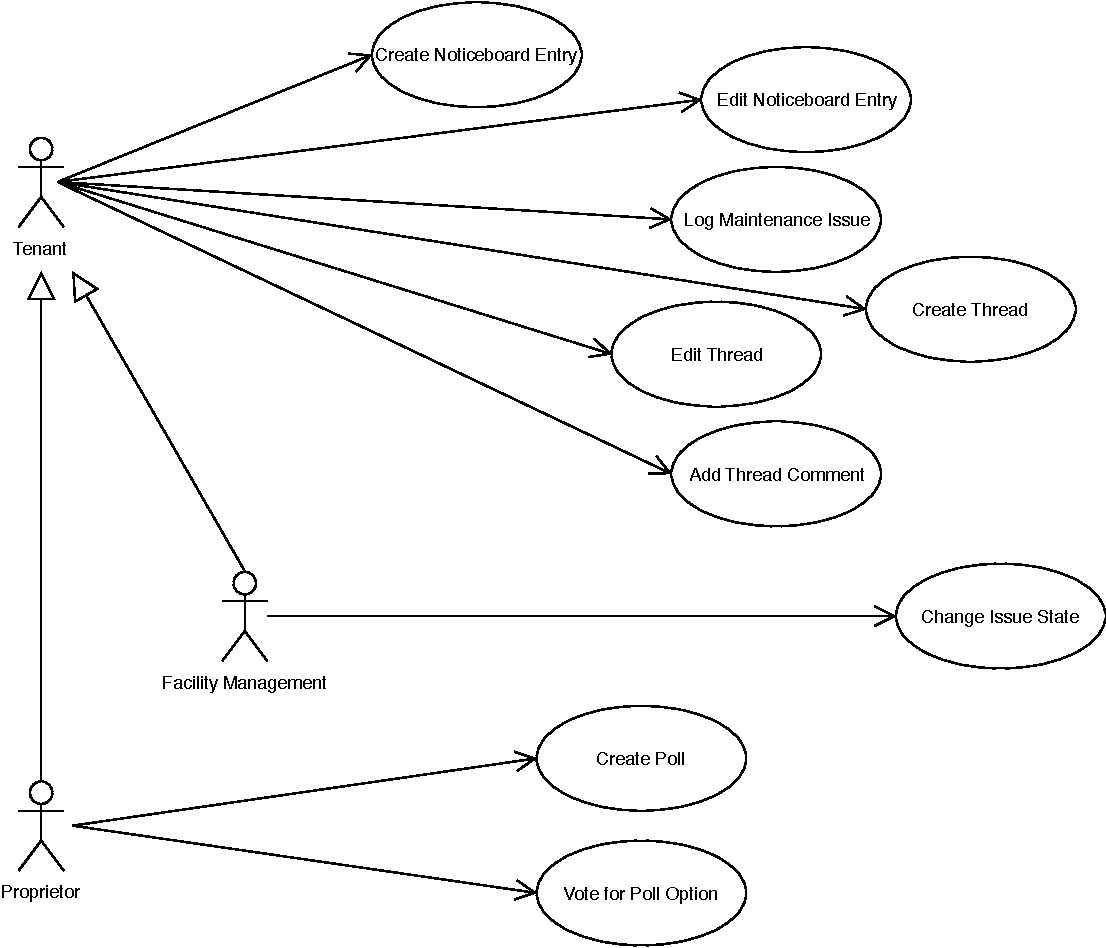
\includegraphics[height=4in,width=4in]{usecases}
    \end{center}
    \caption{Proprietors Assembly Use Cases}
    \label{fig:usecases}
\end{figure}

\section{Potential Solutions}
% Single Page Application because interactive and functionality easy to integrate, smooth native-like feeling
% Using Vue because flexibility and ease of learning were important



\section{Tools and Techniques}

\section{Legal and Ethical Issues}